\section{Criação do \textit{dataset}}
\label{sec:metodologia-datasets}

Conforme introduzimos acima, o primeiro passo para que possamos desenvolver e avaliar a abordagem proposta consiste em definir um conjunto de dados que viabilize isso. Como a proposta apresentada aqui é nova e, devido a isso, não há \textit{dataset}s diretamente compatíveis com ela, optamos por derivar um novo \textit{dataset} a partir de outro já existente -- o \acrfull{asllvd}.

O \acrshort{asllvd} consiste em um amplo \textit{dataset} público\footnote{Disponível em \url{http://www.bu.edu/asllrp/av/dai-asllvd.html}} da \acrshort{asl} que contém aproximadamente 2.745 sinais representados em cerca de 9.763 sequências de vídeo articuladas por indivíduos Surdos nativos. Suas amostras são capturadas por meio de quatro câmeras sincronizadas: uma visão frontal de alta resolução a meia velocidade, outra visão frontal de resolução total, uma visão lateral e uma visão da face, conforme ilustrado na \autoref{fig:asllvd-example}~\cite{athitsos-2008-asllvd,neidle-2012-asllvd}.

\begin{figure}[ht!]
    \centering
    \caption{\textmd{Exemplo de três perspectivas sincronizadas providas pelo \acrshort{asllvd} para o sinal MERRY-GO-ROUND: 
    vista frontal (\subref{subfig:asllvd-example-front}), 
    vista lateral (\subref{subfig:asllvd-example-side}) e 
    vista da face (\subref{subfig:asllvd-example-close}).}}
    \subcaptionbox{\label{subfig:asllvd-example-front}}{
        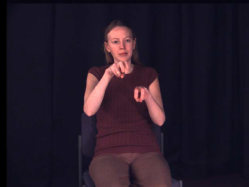
\includegraphics[width=0.25\textwidth]{capitulos/metodologia/imagens/asllvd_example_front}
    }%
    \hfill
    \subcaptionbox{\label{subfig:asllvd-example-side}}{
        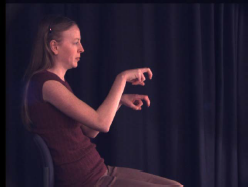
\includegraphics[width=0.25\textwidth]{capitulos/metodologia/imagens/asllvd_example_side}
    }%
    \hfill
    \subcaptionbox{\label{subfig:asllvd-example-close}}{
        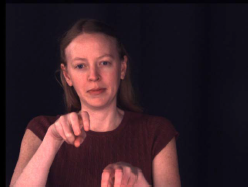
\includegraphics[width=0.25\textwidth]{capitulos/metodologia/imagens/asllvd_example_close}
    }%
    \nomefonte[p. 2]{athitsos-2008-asllvd}
    \label{fig:asllvd-example}
\end{figure}


Para computar parâmetros fonológicos a partir dos frames das amostras do \acrshort{asllvd}, compostos essencialmente de imagens RGB bidimensionais, precisamos realizar um processo de duas etapas: primeiro, estimamos as coordenadas 2D dos esqueletos dos sinalizadores para duas câmeras distintas, frame-a-frame, e as combinamos para projetar um esqueleto no espaço 3D -- isso deu origem ao \textit{dataset} intermediário chamado ASL-Skeleton3D; em seguida, aplicamos um conjunto de operações algébricas sob o esqueleto 3D para calcular os parâmetros fonológicos -- o que gerou assim o nosso \textit{dataset} final chamado ASL-Phono.

Como pode-se imaginar, esse processo envolveu alguns desafios computacionais, entre os quais enumeram-se :

\begin{enumerate}
    \item Definição de abordagens para representar indivíduos no espaço 3D utilizando apenas frames de vídeo simples em 2D do \acrshort{asllvd}, bem como para lidar com as amostras ausentes ou de baixa qualidade encontradas nesse \textit{dataset}.

    \item Estabelecimento de um subconjunto de atributos fonológicos iniciais que pudessem capturar e representar variações significativas no corpo dos indivíduos para o reconhecimento dos sinais, mas que também pudessem ser modelados computacionalmente.
    
    \item Identificação de técnicas matemáticas e medidas antropométricas que suportassem o cálculo e a modelagem dos atributos selecionados.
    
    \item Disponibilização de recursos computacionais significativos para viabilizar o processamento de mais de 9.000 amostras contidas em cada \textit{dataset}, as quais envolveram duas câmeras distintas. Para isso, foram consumidas cerca 40 horas contínuas de processamento em cluster dispondo de CPU e GPU, e gerados mais de 1 TB de dados cada vez que ambos \textit{dataset}s precisaram ser completamente processados.
\end{enumerate}


% Dataset 3d
\subsection{ASL-Skeleton3D}
\label{sec:metodologia-datasets-3d}

O ASL-Skeleton3D é um \textit{dataset} intermediário que introduz a representação em coordenadas 3D das amostras do \acrshort{asllvd}. Esse tipo de representação fornece detalhes mais precisos acerca do corpo dos indivíduos enquanto eles articulam os sinais, o que possibilita a pesquisadores em \acrshort{slr} extrair diferentes tipos de \textit{features}, explorar novas técnicas, ou ainda derivar outros novos \textit{datasets}.

Para que fosse possível projetar as amostras do \acrshort{asllvd} dentro do espaço tridimensional, adotamos uma estratégia que consiste essencialmente em combinar duas de suas perspectivas 2D perpendiculares entre si -- a vista frontal e a vista lateral -- para reconstruir uma perspectiva 3D, conforme ilustra a \autoref{fig:our-strategy-3d}. Com isso, assumimos que enquanto a vista frontal nos fornece os eixos \(x\) e \(y\), a vista lateral nos fornecerá a dimensão de profundidade, correspondente ao eixo \( z\).


\begin{figure}[ht!]
    \centering
    \caption{\textmd{Estratégia adotada para representar as amostras no espaço 3D: as perspectivas frontal (\subref{subfig:our-strategy-3d-front}) e lateral (\subref{subfig:our-strategy-3d-side}) são posicionadas perpendicularmente para reconstruir uma perspectiva 3D (\subref{subfig:our-strategy-3d-persp})}}
    \borda[0.80\textwidth]{
        \subcaptionbox{\label{subfig:our-strategy-3d-front}}{
            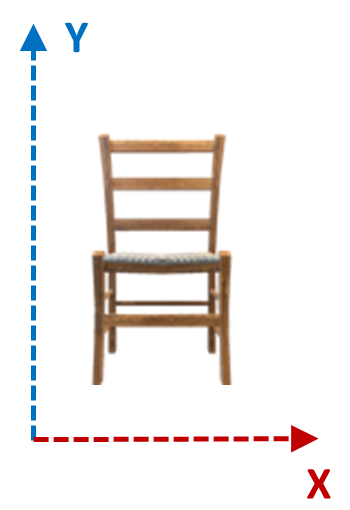
\includegraphics[height=3.5cm]{capitulos/metodologia/imagens/chair_front}
        }%
        \hfill
        \subcaptionbox{\label{subfig:our-strategy-3d-side}}{
            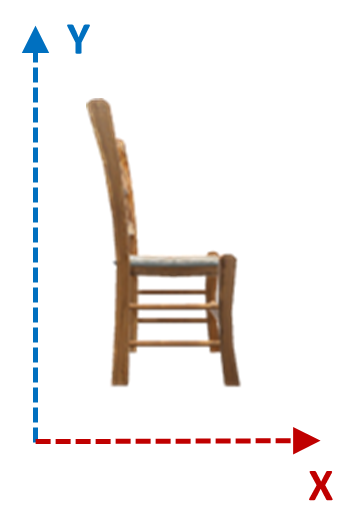
\includegraphics[height=3.5cm]{capitulos/metodologia/imagens/chair_side}
        }%
        \hfill
        \subcaptionbox{\label{subfig:our-strategy-3d-persp}}{
            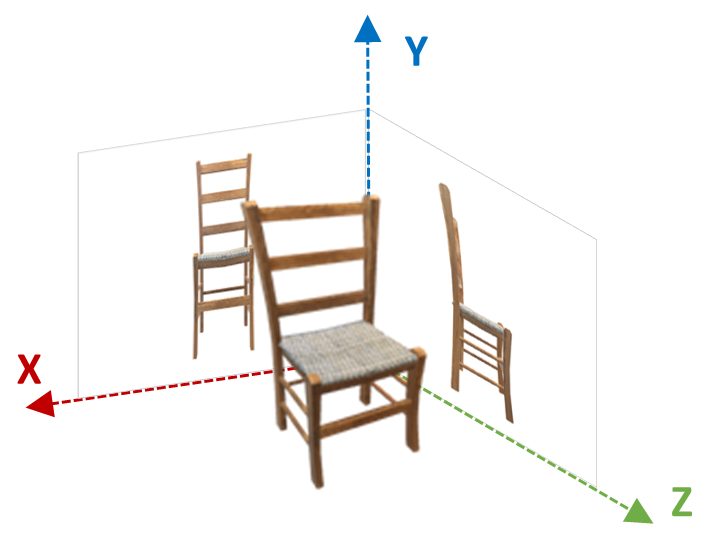
\includegraphics[height=3.5cm]{capitulos/metodologia/imagens/chair_perspective}
        }%
    }
    \nomefonte{}
    \label{fig:our-strategy-3d}
\end{figure}


Uma vez definida essa estratégia, nos baseamos no processo descrito por \citeonline{amorim-2019-stgcn-sl} para realizar a estimativa dos esqueletos para os indivíduos nas amostras. Esse processo é composto pelas etapas de obtenção de amostras, segmentação dos sinais, estimativa e normalização dos esqueletos, as quais sofreram adaptações no contexto do presente trabalho para acomodar a composição de esqueletos 3D e os desafios que encontramos para isso. Discutiremos a seguir as adaptações aplicadas:

% Os passos utilizados para gerar o ASL-Skeleton3D basearam-se no processamento realizado por \citeonline{amorim-2019-stgcn-sl} na construção de um \textit{dataset} de esqueletos 2D da \acrshort{asl}. De um modo geral, eles envolvem a obtenção das amostras, a segmentação dos sinais, a estimativa e a normalização dos esqueletos. Apesar disso, várias adaptações foram necessárias a cada passo para acomodar a estratégia descrita acima e lidar com os desafios encontrados aqui, conforme discutiremos a seguir:

\begin{enumerate}
    \item \textbf{Obtenção das amostras}: nessa etapa as amostras de vídeos são recuperadas a partir dos servidores do \acrshort{asllvd}, mas no contexto atual fazemos isso para ambas as câmeras frontal e lateral.

          A saber, existem dois formatos nos quais os vídeos dessas câmeras podem ser disponibilizados: o \textit{mov}, que é compacto e mais fácil de processar; e o \textit{.vid}, que consiste no vídeo bruto, que é maior e mais pesado para baixar e processar.
          Ao analisar as amostras, identificamos que parte delas possuía ambas câmeras disponíveis nos dois formatos; para outras, cada câmera estava em um formato distinto; contudo, nos piores casos uma das câmeras estava ausente ou corrompida, fazendo com que essas amostras fossem perdidas. Lidar com essa falta de homogeneidade acrescentou uma complexidade inesperada, mas que foi contornada resultando numa perda de apenas 0,16\% das amostras originais -- ou seja, 16 amostras de um total inicial de 9.763.


    \item \textbf{Segmentação dos sinais}: compreende a segmentação das sequências de vídeos do \acrshort{asllvd} em pedaços menores, contendo um único sinal.
          Nessa etapa também reduzimos a taxa de quadros de 60 para 3 FPS, uma vez que consideramos que é pouco provável a articulação de mais de três movimentos relevantes em um único segundo.
          Isso contribuiu para reduzir em cerca de 20 vezes o número de frames a serem processados nas etapas seguintes.


    \item \textbf{Estimativa dos esqueletos 3D}: nesse momento os esqueletos dos sinalizadores são estimados utilizando-se o OpenPose para ambas as câmeras frontal e lateral. Dois esqueletos 2D são obtidos a partir disso:

          \begin{enumerate}
              \item \textit{Esqueleto frontal} (\autoref{subfig:front-side-persp-skeletons-front}), contendo as coordenadas plotadas sobre o eixos \(x\) e \(y\) que correspondem às mesmas coordenadas \(x\) e \(y\) de quando imaginamos o indivíduo representado no espaço tridimensional (vide \autoref{subfig:front-side-persp-skeletons-persp}).
                    % Essas coordenadas descrevem a mesma visão frontal que esperamos obter ao imaginar o nosso esqueleto 3D final observado de frente. Por conta disso, utilizamos essas coordenadas \(x\) e \(y\) da forma como são fornecidas para ancorar o indivíduo no espaço tridimensional. Precisaremos apenas adicionar a dimensão de profundidade.

              \item \textit{Esqueleto lateral} (\autoref{subfig:front-side-persp-skeletons-side}), que também é estimado com um par de coordenadas \(x\) e \(y\) mas que, quando posicionados perpendicularmente ao esqueleto frontal (vide \autoref{subfig:front-side-persp-skeletons-persp}), denotam a dimensão de profundidade e correspondem aos eixos \(z\) e \(y\) do indivíduo no espaço tridimensional, respectivamente. Uma vez que \(y\) já foi obtido por meio do esqueleto frontal, ele pode ser então descartado.

                    % No entanto, vamos aplicar a estratégia descrita acima e posicioná-lo perpendicularmente ao esqueleto frontal (como no ~\autoref{subfig:front-side-persp-skeletons-persp}). Nesse caso, observamos que embora o eixo \(y\) fornecido aqui contenha as mesmas coordenadas que no esqueleto frontal, o eixo \(x\) descreverá coordenadas equivalentes às de profundidade. Dessa forma, tomaremos o eixo \(x\) do esqueleto lateral como sendo o eixo \(z\) (eixo de profundidade) para o nosso esqueleto 3D final.
          \end{enumerate}

          Dessa forma, combinamos as coordenadas \(x\), \(y\) e \(z\) obtidas para dar origem ao nosso esqueleto 3D.

          \begin{figure}[ht!]
              \centering
              \caption{\textmd{Os esqueletos 2D frontal (\subref{subfig:front-side-persp-skeletons-front}) e lateral (\subref{subfig:front-side-persp-skeletons-side}) são posicionados perpendicularmente (\subref{subfig:front-side-persp-skeletons-persp}) e combinados para compor o esqueleto 3D final utilizado aqui}}
              \borda[0.85\textwidth]{
                  \subcaptionbox{\label{subfig:front-side-persp-skeletons-front}}{
                      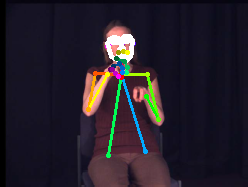
\includegraphics[height=2.5cm]{capitulos/metodologia/imagens/asllvd_example_front_skeleton}
                  }%
                  \hfill
                  \subcaptionbox{\label{subfig:front-side-persp-skeletons-side}}{
                      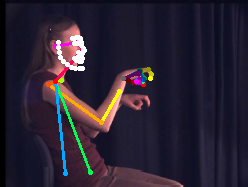
\includegraphics[height=2.5cm]{capitulos/metodologia/imagens/asllvd_example_side_skeleton}
                  }%
                  \hfill
                  \subcaptionbox{\label{subfig:front-side-persp-skeletons-persp}}{
                      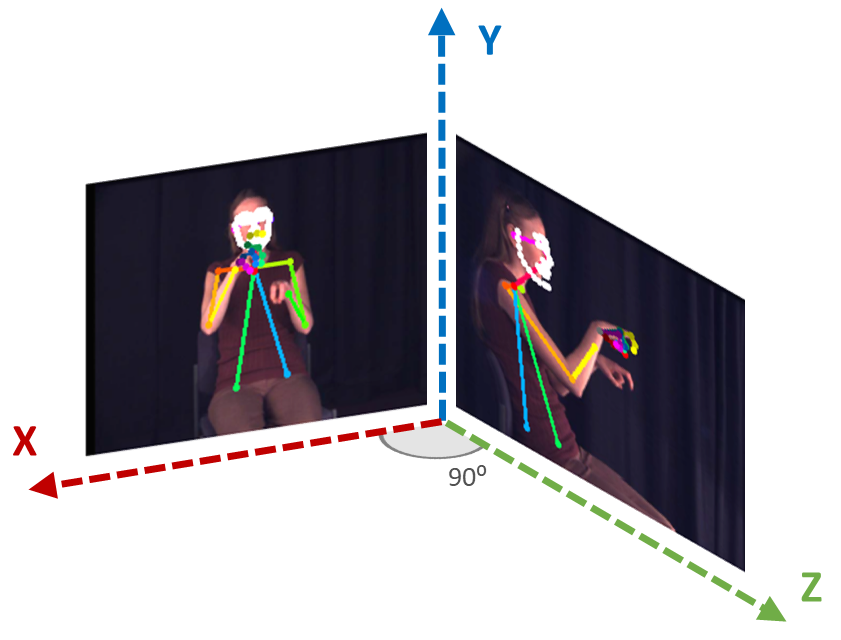
\includegraphics[height=4.0cm]{capitulos/metodologia/imagens/asllvd_front_side_perspective_skeleton}
                  }%
              }
              \nomefonte{}
              \label{fig:front-side-persp-skeletons}
          \end{figure}


    \item \textbf{Normalização dos esqueletos 3D}: por fim, os esqueletos 3D são normalizados para remover variações decorrentes do posicionamento das câmeras e dos corpos dos indivíduos. Isso é importante porque o \acrshort{asllvd} foi capturado através de diferentes seções e envolveu diferentes sinalizadores.

          Adotamos como referência para essa normalização a largura entre os ombros dos sinalizadores (vide \autoref{fig:shoulders-width}), a qual foi inspirada pela medida antropométrica de \textit{diâmetro biacromial} apresentada por \citeonline{stoudt-1970-skinfolds}. Dessa forma, a largura entre os ombros \(W_{shoulders}\) é definida aqui como a distância euclidiana \(d\) entre as coordenadas do ombro esquerdo \(S_{l}\) e do ombro direito \(S_ {r}\), conforme \autoref{eqn:shoulders-width}:

          \figura
          {fig:shoulders-width} % Label
          {capitulos/metodologia/imagens/shoulders_width} % Path
          {height=3.5cm} % Size
          {A largura entre ombros foi utilizada para normalizar as coordenadas nos esqueletos 3D} % Caption
          {} % Citation

          \begin{equation}
              \label{eqn:shoulders-width}
              W_{shoulders} = d\left(S_{l}, S_{r}\right)
          \end{equation}

          Utilizando-se \(W_{shoulders}\) é possível transformar as coordenadas \(K\) do esqueleto 3D em coordenadas normalizadas \(K_{norm}\), conforme \autoref{eqn:normalized-keypoint}:

          % Normalização de pontos-chave:
          \begin{equation}
              \label{eqn:normalized-keypoint}
              K_{norm} = \frac{K}{W_{shoulders}}
          \end{equation}

\end{enumerate}


A \autoref{fig:sample-json-datasetTD} exemplifica uma amostra do ASL-Skeleton3D resultante do processamento acima, bem como suas propriedades. Observa-se no início do arquivo informações básicas extraídas do \acrshort{asllvd}, como rótulo, nome do indivíduo, sessão, cena, frames de início e fim, entre outras. Na propriedade ``frames'' estão listados os frames para aquela sequência e o esqueleto 3D estimado para cada um deles. Cada esqueleto contém grupos referentes ao ``\textit{body}'' (corpo), ``\textit{face}'' (face), ``\textit{hand left}'' (mão direita) e ``\textit{hand right}'' (mão esquerda) que, por sua vez, contêm propriedades que listam o nome da coordenada, o ``\textit{score}'' (ou acurácia) de sua estimativa e os respectivos eixos \(x\), \(y\) e \(z\).
Por exemplo, se observarmos o primeiro índice das propriedades do grupo ``\textit{body}'' veremos que ele corresponde à coordenada ``\textit{nose}'' (nariz), apresenta um \textit{score} de aproximadamente 90\% e coordenadas \(x\), \(y\) e \(z\) localizadas em 4,488, 1,696 e 2,872.

\figura
{fig:sample-json-datasetTD} % Label
{capitulos/metodologia/imagens/code_3d} % Path
{width=0.7\linewidth} % Size
{Exemplo de amostra do ASL-Skeleton3D} % Caption
{} % Citation

O \textit{dataset} final e o código-fonte utilizado para o processamento apresentado nesta seção estão disponíveis publicamente na URL listada abaixo\footnote{Disponível em \url{http://www.cin.ufpe.br/~cca5/asl-skeleton3d}}.


% Dataset phono
\subsection{ASL-Phono}
\label{sec:metodologia-datasets-phono}

O ASL-Phono é um \textit{dataset} que introduz uma nova representação baseada na linguística da língua de sinais, a qual descreve os sinais do \acrshort{asllvd} em termos de seus atributos fonológicos. Para computá-los, foram utilizadas as coordenadas 3D fornecidas pelo ASL-Skeleton3D, o que nos forneceu 9.747 amostras e cerca de 2.650 sinais para novo \textit{dataset}.

Como trata-se de uma versão inicial da representação proposta, optamos por selecionar um subconjunto de quatro parâmetros fonológicos dentre aqueles discutidos na \autoref{sec:linguistica-fonologia}, os quais podem ser expandidos em incrementos futuros desta pesquisa. Esses parâmetros incluem a configuração de mão, o movimento da mão, a orientação da palma e uma expressão não-manual refente à abertura da boca, conforme discutiremos a seguir:

\begin{enumerate}
    \item \textbf{Configuração de mão}: refere-se à configurações das mãos do sinalizador durante a articulação dos sinais.
    O \acrshort{asllvd} fornece a configuração de mão inicial e final para cada um de seus sinais, a qual é definida dentre 88 opções apresentadas pelo \acrfull{asllrp}\footnote{Disponível em \url{http://www.bu.edu/asllrp}} \cite{neidle-2020-asllrp}.

    Utilizamos essa informação como base para computar as configurações de mãos no ASL-Phono, mas tivemos que adotar um passo extra para que pudéssemos atribuir configurações a todos os frames das amostras a partir dessas duas únicas providas. Nesse caso, dividimos os frames em duas metades: a primeira, contendo os frames iniciais do sinal, recebeu a configuração de mão inicial provida pelo \acrshort{asllvd}; a segunda, referente aos frames restantes finais, recebeu a configuração final provida.

    % -----
    \item \textbf{Orientação}: refere-se à direção para qual as palmas das mãos apontam durante a articulação dos sinais.
    Para calculá-la, utilizamos um pouco de álgebra linear e exploramos a relação das mãos para com o espaço tridimensional em que suas coordenadas estão representadas \cite{anton-2013-algebra}.

    Para isso, primeiro assumimos cada palma como sendo um plano que atravessa as coordenadas estimadas para as mãos (vide \autoref{subfig:palm-orientation}). A partir disso, selecionamos três coordenadas para descrever este plano: \(W\), que corresponde à coordenada do pulso; \(L\), localizada na base do dedo mínimo; e \(I\), localizada na base do dedo indicador.

    \begin{figure}[ht!]
        \centering
        \caption{
            \textmd{As coordenadas \(W\), \(L\) e \(I\) e os vetores auxiliares são utilizados para obter a normal \(\protect \overrightarrow{n}\) da palma da mão~(\subref{subfig:palm-orientation}).
            A direção da palma \(O_{palm}\) é então calculada a partir de \(\protect \overrightarrow{n}\) e descrita dentre um conjunto de direções possíveis~(\subref{ subfig:palm-directions}).}
        }
        \subcaptionbox{\label{subfig:palm-orientation}}{
            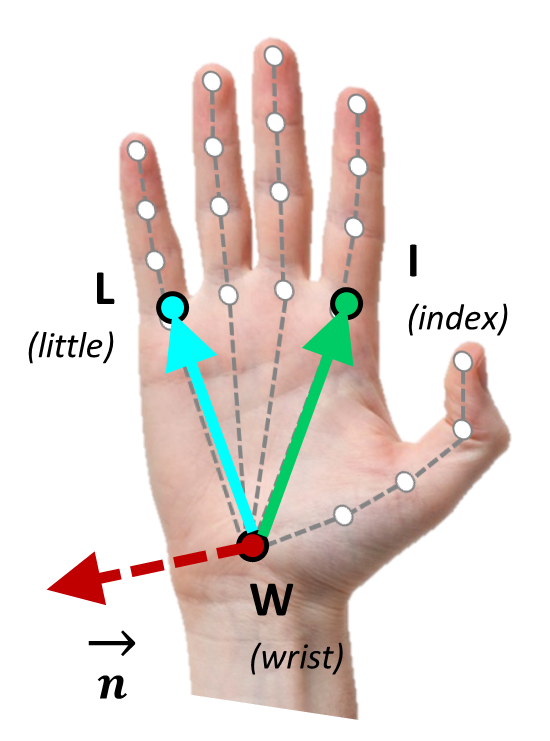
\includegraphics[height=4cm]{capitulos/metodologia/imagens/palm_orientation_algebra}
        }%
        \hspace{1cm}
        \subcaptionbox{\label{ subfig:palm-directions}}{
            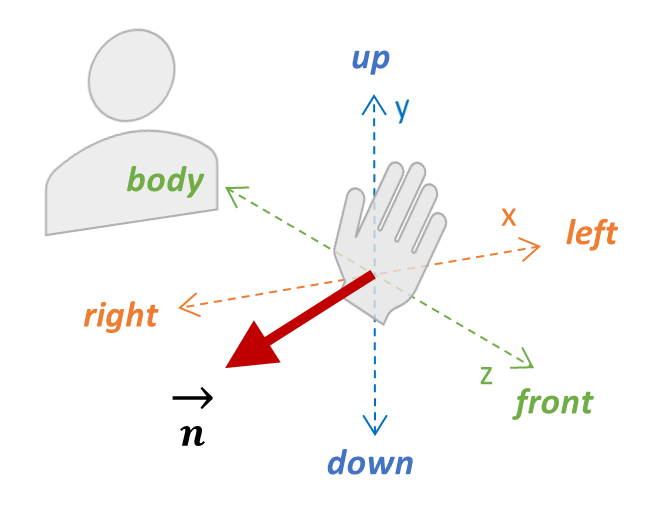
\includegraphics[height=4cm]{capitulos/metodologia/imagens/hand_orientations}
        }%
        \nomefonte{}
        \label{fig:palm-orientation-directions}
    \end{figure}

    Por meio dessas coordenadas, é possível estabelecer dois vetores para descrever o plano da palma (vide \autoref{subfig:palm-orientation}): \(\overrightarrow{WL}\), indicado pela seta azul e \(\overrightarrow{WI}\), indicado pela seta verde. Através deles, é possível estabelecer o vetor normal \(\overrightarrow{n}\) perpendicular ao plano da palma, que é indicado pela seta vermelha tracejada, e calculado conforme \autoref{eqn:normal-palm-left} (para a mão esquerda) e \autoref{eqn:normal-palm-right} (para a mão direita):

    % Palm orientation:
    \begin{equation}
        \label{eqn:normal-palm-left}
        \overrightarrow{n}_{left} = \overrightarrow{WI} \times \overrightarrow{WL}
    \end{equation}

    \begin{equation}
        \label{eqn:normal-palm-right}
        \overrightarrow{n}_{right} = \overrightarrow{WL} \times \overrightarrow{WI}
    \end{equation}


    Finalmente, ao avaliar os valores dos eixos \(x\), \(y\) e \(z\) da normal \(\overrightarrow{n}\), é possível definir a orientação da palma \(O_{palm}\) como sendo a combinação de até três direções, cujas opções são: \textit{right} (direita), \textit{left} (esquerda), \textit{up} (para cima), \textit{down} (para baixo), \textit{body} (para o corpo) ou \textit{front} (para frente).
    Por exemplo, ``\textit{right\_down}'' e ``\textit{left\_up\_body}'' seriam orientações válidas. Essa avaliação é realizada conforme \autoref{eqn:palm-orientation-directions}:
    
    % Directions
    \begin{equation}
        \label{eqn:palm-orientation-directions}
        O_{palm} =
        \begin{cases}
            right & \text{if $\overrightarrow{n}_x < {-k}$ } \\
            left  & \text{if $\overrightarrow{n}_x > {k}$ }  \\
            up    & \text{if $\overrightarrow{n}_y < {-k}$ } \\
            down  & \text{if $\overrightarrow{n}_y > {k}$ }  \\
            body  & \text{if $\overrightarrow{n}_z < {-k}$ } \\
            front & \text{if $\overrightarrow{n}_z > {k}$ }  \\
        \end{cases}
    \end{equation}

    Onde o limiar \(k\) é definido empiricamente como 0,30 para filtrar variações pouco significativas em \(\overrightarrow{n}\). Observe na \autoref{ subfig:palm-directions} como essa operação é aplicada no espaço tridimensional à frente do sinalizador.


    % -----
    \item \textbf{Movimento}: descreve o deslocamento realizado pelas mãos na articulação do sinal.
    De forma semelhante ao que fizemos para a orientação da palma, aqui também analisaremos coordenadas das mãos para determinar sua trajetória no espaço.

    Para isso, utilizaremos a coordenada \(M\) como ponto de referência para as mãos, a qual está localizada na base do dedo médio (vide \autoref{fig:hand-movement-directions}). Com base nela, calcularemos o deslocamento ocorrido entre os frames anterior (tempo \(t-1\)) e atual (tempo \(t\)) para determinar o vetor de movimento \(\overrightarrow{m}\) (indicado pela seta vermelha tracejada), conforme \autoref{eqn:hand-movement}:
    
    % Movement of the hands:
    \begin{equation}
        \label{eqn:hand-movement}
        \overrightarrow{m} = M_{t} - M_{t-1}
    \end{equation}

    \begin{figure}[ht!]
        \centering
        \caption{
            \textmd{O vetor de movimento \(\protect \overrightarrow{m}\) é calculado pela trajetória da coordenada \(M\) entre os frames anterior (\(t-1\)) e atual (\(t\))~(\subref{subfig:hand-movement}).
            O movimento da mão \(V_{hand}\) é então obtido a partir de \(\protect \overrightarrow{m}\) e descrito dentre um conjunto de direções possíveis~(\subref{subfig:hand-directions}).}
        }
        \subcaptionbox{\label{subfig:hand-movement}}{
            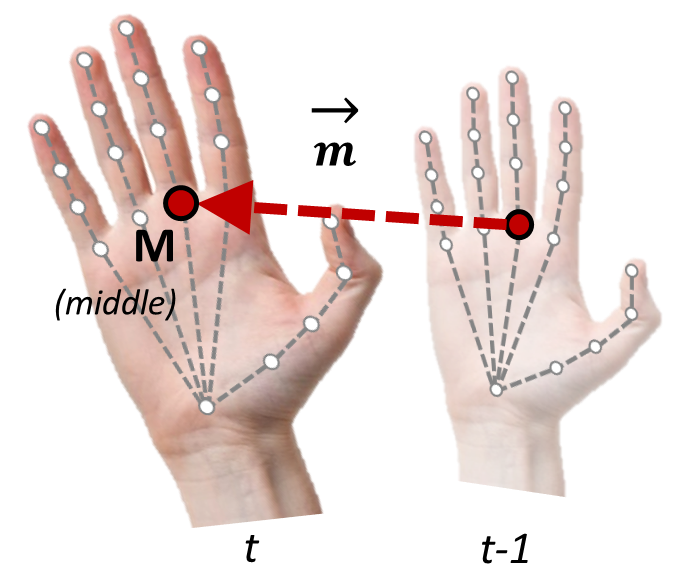
\includegraphics[height=4cm]{capitulos/metodologia/imagens/hand_movement}
        }%
        \hspace{1cm}
        \subcaptionbox{\label{subfig:hand-directions}}{
            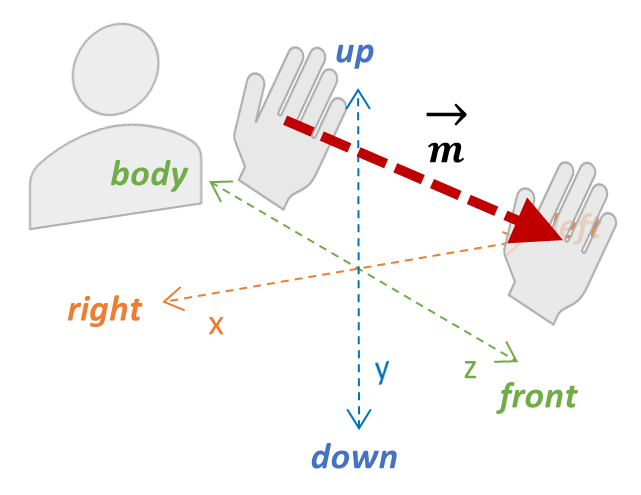
\includegraphics[height=4cm]{capitulos/metodologia/imagens/hand_movement_2}
        }%
        \nomefonte{}
        \label{fig:hand-movement-directions}
    \end{figure}


    A partir do vetor \(\overrightarrow{m}\), aplicamos uma operação parecida com a que foi utilizada para a orientação da mão, para definir o movimento da mão \(V_{hand}\) como a combinação de até três direções, cujas opções são: \textit{right} (direita), \textit{left} (esquerda), \textit{up} (para cima), \textit{down} (para baixo), \textit{body} (para o corpo) ou \textit{front} (para frente). Essa operação é detalhada na \autoref{eqn:hand-movement-directions} e a \autoref{subfig:hand-directions} ilustra ela segundo a perspectiva do sinalizador:

    % Directions
    \begin{equation}
    \label{eqn:hand-movement-directions}
        V_{hand} =
            \begin{cases}
                right & \text{if $\overrightarrow{m}_x < {-k}$ }\\
                left  & \text{if $\overrightarrow{m}_x > {k}$ }\\
                up    & \text{if $\overrightarrow{m}_y < {-k}$ }\\
                down  & \text{if $\overrightarrow{m}_y > {k}$ }\\
                body  & \text{if $\overrightarrow{m}_z < {-k}$ }\\
                front & \text{if $\overrightarrow{m}_z > {k}$ }\\
            \end{cases}    
    \end{equation}

    Aqui o limiar \(k\) também foi definido como 0,30 para remover movimentos pouco significantes.


    % -----
    \item \textbf{Expressão não-manual - abertura da boca}: refere-se à abertura da boca, a cada frame, a qual pode prover significado adicional ao sinal.
    Para calculá-lo, nos baseamos no trabalho de \citeonline{ferrario-2000-study-lips}, o qual analisa e propõe algumas medidas antropométricas para os lábios.

    Dentre essas medidas apresentadas, selecionamos a \textit{vermilion height to mouth width} (ou altura dos lábios com relação à largura da boca), visto que ela é capaz de capturar a abertura dos lábios em termos de uma única proporção. A altura dos lábios é dada pela distância \(d\) entre o \textit{labiale superius} \(LS\) e o \textit{labiale inferius} \(LI\), que são as coordenadas mais externas dos lábios superior e inferior. A largura da boca, por sua vez, é a distância \(d\) entre o \textit{cheilion direito} \(CH_r\) e o \textit{cheilion esquerdo} \(CH_l\), que são as coordenadas do lado direito e esquerdo da boca (vide \autoref{fig:mouth-openness}).

    \figura
        {fig:mouth-openness} % Label
        {capitulos/metodologia/imagens/mouth_openness} % Path
        {height=4cm} % Size
        {A abertura da boca foi calculada com base na medida \textit{vermilion height to mouth width} (ou altura dos lábios com relação à largura da boca) apresentada por \cite{ferrario-2000-study-lips}, a qual considera as coordenadas \(LS\), \(LI\), \(CH_r\) e \(CH_l\).} % Caption
        {ferrario-2000-study-lips} % Citation

        
    Sendo assim, a abertura de boca \(P_{mouth}\) pode ser então definida como na \autoref{eqn:mouth-openness}:

    % Abertura da boca:
    \begin{equation}
        \label{eqn:mouth-openness}
        P_{mouth} = \frac{d(LS, LI)}{d(CH_r, CH_l)}
    \end{equation}

\end{enumerate}


% Estatísticas:
Na \autoref{tab:dataset-phono-stats}, podemos observar algumas estatísticas calculadas a partir do ASL-Phono, que nos permitem compreender como as amostras ficaram organizadas no \textit{dataset} após o processamento acima. 
Nela, os números são listados segundo três perspectivas: 

\begin{itemize}
    \item \textit{Dataset} inteiro: contabiliza o número total de amostras, sinais, movimentos distintos, entre outros, para todo o \textit{dataset}. Por exemplo, pode-se ler que o \textit{dataset} possui 9.747 amostras, 2.650 sinais e 26 movimentos para a mão dominante.
    
    \item Por amostra: contém estatísticas de números mínimos, máximos, médios e desvio padrão para os parâmetros computados acima. Por exemplo, lê-se que, em média, as amostras possuem 3,02 frames, sendo que a mais curta contém apenas 1 frame e a mais longa possui 12 frames. De maneira semelhante, as amostras têm em média de 1,94 movimentos e 2,20 orientações de mão distintas para a mão dominante.

    \item Por sinal: contém estatísticas de números mínimos, máximos, médios e desvio padrão para os sinais contidos no \textit{dataset}. Por exemplo, lê-se que cada sinal possui em média de 3,68 amostras, sendo que alguns deles possuem apenas 1 e outros possuem valores atípicos de 59 amostras (a considerar pelo desvio padrão apresentado). Além disso, cada sinal apresenta em média 6,04 movimentos e 5,37 orientações de mão distintas para a mão dominante.
\end{itemize}

% Please add the following required packages to your document preamble:
% \usepackage{multirow}
% \usepackage{graphicx}
% \usepackage[table,xcdraw]{xcolor}
% If you use beamer only pass "xcolor=table" option, i.e. \documentclass[xcolor=table]{beamer}
\begin{table}[]
    \centering
    \caption{Estatísticas calculadas a partir do ASL-Phono, as quais são visualizadas para todo o \textit{dataset} e segundo agrupamentos por amostra e por sinal. (D) refere-se à mão dominante e (ND) refere-se à mão não-dominante.}
    \label{tab:dataset-phono-stats}
    \resizebox{0.9\textwidth}{!}{%
        \begin{tabular}{cr|ccc|ccccccc}
            \hline
            \rowcolor[HTML]{EFEFEF}
                                                                                     &        & \cellcolor[HTML]{EFEFEF}                           & \cellcolor[HTML]{EFEFEF}                         & \cellcolor[HTML]{EFEFEF}                         & \multicolumn{2}{c}{\cellcolor[HTML]{EFEFEF}Movimento} & \multicolumn{2}{c}{\cellcolor[HTML]{EFEFEF}Orientação} & \multicolumn{2}{c}{\cellcolor[HTML]{EFEFEF}Config. mão} & \cellcolor[HTML]{EFEFEF}                                                                                                                       \\
            \rowcolor[HTML]{EFEFEF}
                                                                                     &        & \multirow{-2}{*}{\cellcolor[HTML]{EFEFEF}Amostras} & \multirow{-2}{*}{\cellcolor[HTML]{EFEFEF}Sinais} & \multirow{-2}{*}{\cellcolor[HTML]{EFEFEF}Frames} & (D)                                                   & (ND)                                                   & (D)                                                     & (ND)                     & (D)  & (ND) & \multirow{-2}{*}{\cellcolor[HTML]{EFEFEF}\begin{tabular}[c]{@{}c@{}}Abertura \\ da boca\end{tabular}} \\ \hline
            \begin{tabular}[c]{@{}c@{}}Dataset \\ inteiro\end{tabular}               &        & 9.747                                              & 2.650                                            & -                                                & 26                                                    & 26                                                     & 26                                                      & 26                       & 85   & 78   & -                                                                                                     \\ \hline
                                                                                     & Mín    & -                                                  & -                                                & 1                                                & 0                                                     & 0                                                      & 0                                                       & 0                        & 0    & 0    & 0,01                                                                                                  \\
                                                                                     & Máx    & -                                                  & -                                                & 12                                               & 10                                                    & 8                                                      & 6                                                       & 5                        & 2    & 2    & 2,19                                                                                                  \\
                                                                                     & Média  & -                                                  & -                                                & 3,02                                             & 1,94                                                  & 1,26                                                   & 2,20                                                    & 1,18                     & 1,17 & 0,72 & 0,13                                                                                                  \\
            \multirow{-4}{*}{\begin{tabular}[c]{@{}c@{}}Por \\ amostra\end{tabular}} & Desvio & -                                                  & -                                                & 0,87                                             & 0,83                                                  & 1,15                                                   & 0,79                                                    & 1,07                     & 0,38 & 0,58 & 0,12                                                                                                  \\ \hline
                                                                                     & Mín    & 1                                                  & -                                                & -                                                & 1                                                     & 0                                                      & 1                                                       & 0                        & 1    & 0    & 0,02                                                                                                  \\
                                                                                     & Máx    & 59                                                 & -                                                & -                                                & 24                                                    & 16                                                     & 22                                                      & 14                       & 8    & 8    & 0,99                                                                                                  \\
                                                                                     & Média  & 3,68                                               & -                                                & -                                                & 6,04                                                  & 3,66                                                   & 5,37                                                    & 2,63                     & 1,81 & 1,17 & 0,13                                                                                                  \\
            \multirow{-4}{*}{\begin{tabular}[c]{@{}c@{}}Por \\ sinal\end{tabular}}   & Desvio & 2,67                                               & -                                                & -                                                & 2,93                                                  & 3,18                                                   & 2,29                                                    & 2,35                     & 0,99 & 1,14 & 0,07                                                                                                  \\ \hline
        \end{tabular}%
    }
    \nomefonte{}
\end{table}


% Exemplo de amostra:
As amostras no ASL-Phono possuem uma estrutura semelhante àquela apresentada para o ASL-Skeleton3D. A diferença, no entanto, está na propriedade "frames", que ao invés de listar coordenadas 3D agora inclui os respectivos atributos fonológicos computados para os frames. Cada atributo, por sua vez, contém o seu respectivo valor e pode conter um \textit{score}, que identifica sua acurácia com base na acurácia das coordenadas envolvidas no seu processamento.

\figura
    {fig:sample-json-phono} % Label
    {capitulos/metodologia/imagens/code_phono} % Path
    {width=0.65\linewidth} % Size
    {Exemplo de amostra do ASL-Phono e propriedades fornecidas para ela.} % Caption
    {} % Citation


O \textit{dataset} resultante do processamento acima e o código-fonte utilizado para isso estão disponíveis publicamente na URL listada abaixo\footnote{Disponível em \url{http://www.cin.ufpe.br/~cca5/asl-phono}}.
